\documentclass[8pt,landscape]{scrartcl}
\usepackage[left=1cm,right=1cm,top=1cm,bottom=1cm,landscape]{geometry}
\usepackage[utf8]{inputenc}
\usepackage[ngerman]{babel}
\usepackage{xcolor}
\usepackage{amsfonts}
\usepackage{multicol}
\usepackage{amsmath}
%\usepackage{amsfonts}
%\usepackage{amssymb}
%\usepackage{gensymb}
%\usepackage{dsfont}
\usepackage{calc}
%\usepackage[permil]{overpic}
\usepackage{graphicx}
%\graphicspath{{gfx/}}
\usepackage{blindtext}


\setlength\parindent{0pt}

\author{martinhediger}
\title{Formelsammlung MGLI}
\begin{document}



\setlength{\columnsep}{1cm}
\begin{multicols}{3}
Martin Hediger, FHNW

%\begin{klm}


\section{Zahlenmengen}
%\begin{small}
$\mathbb{N} := \{0, 1, 2, ...\} $ - nat\"urliche Zahlen\\
$\mathbb{Z} := \{..., -2, -1, 0, 1, 2, ...\}$ - ganze Zahlen\\
$\mathbb{Q} := \{\frac{m}{n} | m \in \mathbb{Z} \land n \in \mathbb{N} \land n \neq 0 \}$ - rationale Zahlen\\
$\mathbb{R} := \{x | x \mbox{ als endlicher oder unendlicher Bruch darstellbar} \}$ - reelle Zahlen
%\end{small}



\section{Aussagenlogik}
%\begin{small}

\subsection{Wahrheitstabellen}

\begin{tabular}{ll||c}
A & B & A $\land$ B  \\ \cline{1-3}
0 & 0 &           0  \\
0 & 1 &           0  \\
1 & 0 &           0  \\
1 & 1 &           1
\end{tabular}
\begin{tabular}{ll||c}
A & B & A $\lor$ B  \\ \cline{1-3}
0 & 0 &           0  \\
0 & 1 &           1  \\
1 & 0 &           1  \\
1 & 1 &           1
\end{tabular}
\begin{tabular}{ll||c}
A & B & A $\implies$ B  \\ \cline{1-3}
0 & 0 &           1  \\
0 & 1 &           1  \\
1 & 0 &           0  \\
1 & 1 &           1
\end{tabular}

\begin{tabular}{ll||c}
A & B & A $\iff$ B  \\ \cline{1-3}
0 & 0 &           1  \\
0 & 1 &           0  \\
1 & 0 &           0  \\
1 & 1 &           1
\end{tabular}
\begin{tabular}{ll||c}
A & B & A $XOR$ B  \\ \cline{1-3}
0 & 0 &           0  \\
0 & 1 &           1  \\
1 & 0 &           1  \\
1 & 1 &           0  \\
\end{tabular}

\textbf{Implikation:} Wenn wir sagen $A$ \textit{impliziert} $B$, dann bedeutet dies \textit{``Wenn $A$ wahr ist, dann kann die Aussage, dass dann $B$ falsch ist, nicht mehr wahr sein''.}\\
\textbf{Kontraposition:} $(A \implies B) \equiv (\lnot B \implies \lnot A)$\\
Regen impliziert nasse Strassen.
Trockene Strasse impliziert Sonnenschein.
Nasse Strasse impliziert \textbf{nicht} Regen.
Sonnenschein impliziert \textbf{nicht} trockene Strassen.

%\end{small}

\subsection{Normalformen}
Berechnen mit Wahrheitstabelle oder Rechenregeln.\\

\begin{small}
\begin{tabular}{lll|c | ll}
A & B & C & $f$ & KNF Klausel                      & DNF Klausel                     \\ \cline{1-6} 
0 & 0 & 0 & 0   &  $(A \lor B \lor C)$             & Nicht relevant für DNF          \\
0 & 0 & 1 & 0   &  $(A \lor B \lor \lnot C)$       & Nicht relevant für DNF          \\
0 & 1 & 0 & 1   &  Nicht relevant für KNF          & $(\lnot A \land B \land \lnot C)$ \\
1 & 1 & 0 & 0   &  $(\lnot A \lor \lnot B \lor C)$ & Nicht relevant für DNF          \\
... & & & 
\end{tabular}
\end{small}

\textbf{Konjunktive NF:} $f = f_1 \land f_2 \land \dots$, f\"ur KNF sind wegen den Identit\"atsgesetzen nur die Zeilen massgebend, welche $f$ den Wahrheitswert 0 ($false$) zuordnen (Zeilen die $1$ sind spielen keine Rolle weil $f \land true = f$)\\

\textbf{Disjunktive NF:} $f = f_1 \lor f_2 \lor \dots$\\
Angenommen, $f(0, 1, 0) = 1$, dh die DNF muss für $(0, 1, 0)$ 1 zurückgeben.
Die DNF ($f_1 \lor f_2 \lor ...$) ist $=1$, wenn nur schon eine Klausel $=1$ ist.
Also m\"ussen in der DNF die Argumente der Klausel umgedreht werden (da sie in der Klammer mit $\land$ verkn\"upft sind).



\section{Mengenalgebra}

%\begin{small}
\subsection{Rechenregeln Quantoren}
\begin{tabular}{lll}
Verneinungss\"atze     & & \\
$\lnot (\forall x \in M : A(x))       \iff \exists x \in M : \lnot A(x) $ & & \\
$\lnot (\forall x \in M : \lnot A(x)) \iff \exists x \in M : A(x) $ & & \\
$\lnot (\exists x \in M : A(x)        \iff \forall x \in M : \lnot A(x) $ & & \\
$\lnot (\exists x \in M : \lnot A(x)) \iff \forall x \in M : A(x) $ & & \\
& & \\

Vertauschbarkeitss\"atze & & \\
$ \forall x \in M, y \in N : A(x, y) \iff \forall y \in N, x \in M : A(x, y) $ & & \\
$ \exists x \in M, y \in N : A(x, y) \iff \exists y \in N, x \in M: A(x, y) $ & & \\
$ \exists x \in M : \forall y \in N : A(x, y) \textcolor{red}{\implies} \forall y \in N : \exists x \in M : A(x, y) $ & & \\\\
$ \forall x \in M : A(x) \textcolor{red}{\implies} \exists x \in M : A(x)   $ & & \\
$ \exists ! x \in M : A(x) \textcolor{red}{\implies} \exists x \in M : A(x) $ & &\\
\end{tabular}

\textbf{Sprachgebrauch:}\\
``Einige meiner Freunde sind schlau.'' $\iff$ $\exists x : F(x) \land S(x) $\\
$\exists x : (\forall y : A(x, y))$: ``\textit{Es gibt (mind.) ein Produkt, welches im Korb jeder Person liegt.}''\\
$\forall y : (\exists x : A(x, y))$: ``\textit{Alle Personen haben (mind.) 1 Produkt im Korb.}''\\

\begin{tabular}{l c l}
Verteilungss\"atze & & \\
$\exists x \in M: (P(x) \lor Q(x))$ & $\iff$ & $(\exists x \in M : P(x)) \lor (\exists x \in M : Q(x))$\\
$\exists x \in M: (P(x) \land Q(x))$ & $\implies$ & $(\exists x \in M : P(x)) \land (\exists x \in M : Q(x))$\\
$\forall x \in M: (P(x) \lor Q(x))$ & $\impliedby$ & $(\forall x \in M : P(x)) \lor (\forall x \in M : Q(x))$\\
$\forall x \in M: (P(x) \land Q(x))$ & $\iff$ & $(\forall x \in M : P(x)) \land (\forall x \in M : Q(x))$\\
\end{tabular}



\subsection{Rechenregeln}
\begin{small}
\begin{tabular}{lll}
Operatoren    & $\cap/\cup \to \text{AND/OR} \to \text{Konj/Disj}$ &                  \\
% Dualität      & $\bar{0} = 1$ & \bar{1} = 0$                       \\
Idempotenz    & $A \cap A = A$                          & $A \cup A = A$              \\
Kommutativ    & $A \cap B = B \cap A$                   & $A \cup B = B \cup A$       \\
Identit\"at   & $A \cap G = A$                          & $A \cup \emptyset = A$      \\
              & $A \cap \emptyset = \emptyset$          & $A \cup G = G$              \\
Assoziativ    & $(A \cap B) \cap C = A \cap (B \cap C)$ &                             \\
              & $(A \cup B) \cup C = A \cup (B \cup C)$ &                             \\
Absorption    & $A \cap (A \cup B) = A$                 & $A \cup (A \cap B) = A$     \\
Distributiv   & $A \cap (B \cup B) = (A \cap B) \cup (A \cap C)$ &                    \\
              & $A \cup (B \cap C) = (A \cup B) \cap (A \cup C)$                      \\
De Morgan     & $(A \cap B)^c = A^c \cup B^c$           & $(A \cup B)^c = A^c \cap B^c$ \\
Komplement\"ar& $A \cap A^c= \emptyset$                   & $A \cup A^c = G$            \\
              & $(A^c)^c = A$                           &                             \\
              & $G^c = \emptyset$                       &                             \\
              & $\emptyset^c = G$                       &                             \\
Teilmengen    & $A \subseteq B \implies (A \cap B = A)$ &                             \\
              & $A \subseteq B \implies (A \cup B = B)$ &                             \\
              & $(A \subseteq B ) \land (B \subseteq C) \implies (A \subseteq C)$ &   \\
\end{tabular}
\end{small}

\subsection{Definitionen}
\textbf{Vereinigung:} $A \cup B := \{ x \in G | x \in A \lor x \in B \}$\\
\textbf{Schnitt:}     $A \cap B := \{ x \in G | x \in A \land x \in B \}$\\
\textbf{Differenz:}   $A \setminus B := \{x \in G | (x \in A \land x \not\in B) \}$\\
\textbf{Sym Diff.:}   $A \bigtriangleup B := \{x \in G | (x \in A \land x \not \in B) \lor (x \in B \land x \not \in A) \}$, $A \bigtriangleup B = (A \setminus B) \cup (B \setminus A)$ \\
\textbf{Complement:}  $A^c := \{x \in G | x \not \in A \} = G \setminus A$\\
\textbf{Kart. Produkt:} $A \times B := \{ (x, y) | x \in A \land y \in B \}$\\
\textbf{Teilmenge:} $x \in A \implies x \in B$, dann ist $A \subseteq B$, dh. $A$ ist Teilmenge von $B$ und $B$ ist Obermenge von $A$



%\end{small}


\subsection{Partition}
Alle Partitionen von $\{0, 1, 2\}$:
$\{ \{0\}, \{1\}, \{2\} \}$, $\{ \{0\}, \{1, 2\} \}$, $\{ \{1\}, \{0, 2\} \}$, $\{ \{2\}, \{0, 1\} \}$, $\{ \{0, 1, 2\} \}$.


\subsection{Potenzmenge}
Menge aller Teilmengen einer Menge $A$ wird Potenzmenge genannt.\\
$A := \{ 1, 2, 3 \}$, dann ist $P(A) = \{ \emptyset, \{1\}, \{2\}, \{3\}, \{1, 2\}, \{1, 3\}, \{2, 3\}, A\}$.\\
$P(\emptyset) = \{ \emptyset \} = \{ \{ \} \}$\\
M\"achtigkeit der Potenzmenge einer endlichen Menge ist $\left|P(A)\right| = 2^{|A|}$.\\
\textbf{Beachten:}\\
$(x, y) \in M \times M \implies \{ \{ (x, y) \} \} \subseteq P(M \times M)$\\
$(x, y) \in M \times M \implies \{ (x, y) \} \in P(M \times M)$\\
\textbf{Anzahl Relationen:}\\
$M = \{ 1, 2, 3, 4 \}$ $\rightarrow$ Anzahl Relationen $| P( M \times M ) | = 2^{ |M| \times |M| } = 2^{16}$





\section{Relationen}
%\begin{small}

\begin{bf}Reflexivit\"at:\end{bf} Jeder Knoten hat eine Schleife, $\forall x \in A: (x, x) \in R$.
Kontrollieren: $(x, x) \in R$?\\
\begin{bf}Symmetrie:\end{bf} F\"ur jeden Pfeil gibt es einen Pfeil in Gegenrichtung (Schleifen siend gleichzeitig Pfeil uend Pfeil in Gegenrichtung).
Kontrollieren $(x, y) \in R$ und $(y, x) \in R$?\\
$\forall x, y \in A : \left( (x, y) \in R \implies (y, x) \in R \right)$\\ 
\begin{bf}Antisymmetrie:\end{bf} F\"ur jeden Pfeil, der nicht Schleife ist, gibt es keinen Pfeil in Gegenrichtung.\\
$\forall x, y \in A : \left( x \neq y \land (x, y) \in R \implies (y, x) \not\in R \right)$\\ 
Kontrollieren $(x, y) \in R$ und $(y, x) \not\in R$? Falls ja ist es antisymmetrisch\\
\begin{bf}Transitivit\"at:\end{bf} Jeder Pfad entlang zweier Pfeile (mit gleichem Richtungssinn) hat einen abk\"urzenden Pfeil vom Anfangs- zum Endknoten des Pfades\\
$\forall x, y, z \in A: \left( (x, y) \in R \land (y, z) \in R \implies (x, z) \in R \right)$\\
Beachten: f\"ur Transitivit\"at ist erforderlich mind. zwei Paare $(x, y) \in R$ und $(y, z) \in R$ zu haben, ansonsten w\"are Pr\"amisse der Definition der Implikation nicht erf\"ullt.
Wenn nicht zwei Paare vorhanden sind $\in R$, ist die Relation automatisch transitiv.



\subsection{\"Aquivalenzrelationen}
\begin{bf}Definition:\end{bf} Eine bin\"are Relation $R \subseteq A \times A $ heisst \"Aquivalenzrelation gdw. sie reflexiv, symmetrisch, transitiv ist.\\
Zwei Objekte $x, y \in A$ mit $(x, y) \in R$ heissen dann \"aquivalent zueinander, geschrieben $x \sim y$, oder auch $\sim (x, y)$ wenn $(x, y) \in \sim$ ist.\\
\begin{bf}\"Aquivalenzklasse:\end{bf} $\left[x\right]_{\sim} := \{ y \in A | x \sim y \}$: ``\textit{Jedes Element steht mit jedem in Relation und nicht in Relation mit Elementen ausserhalb der Klasse}.''\\\\ 
\begin{bf}Beispiel:\end{bf} \"Aquivalenzrelation mit drei \"Aquivalenzklassen\\
$x \sim y \iff 3| \left| x - y \right|$ (3 teilt Betrag):\\
$\left[0\right]_{\sim} = \{ 0, 3, 6, 9, ...\}$\\
$\left[1\right]_{\sim} = \{ 1, 4, 7, 10, ...\}$\\
$\left[2\right]_{\sim} = \{ 2, 5, 8, 11, ...\}$\\\\
\"Aquivalenzrelationen partitionieren ihre Menge und sind gegenseitig disjunkt.\\
\textbf{Bell-Zahlen:} 1, 2, 5, 15, 52, ...

\begin{tabular}{lcccc}
            & $<$ & $\leq$ & $\neq$ & = \\\hline
reflexiv    & n   & j      & n      & j \\
symm.       & n   & n      & j      & j \\
antisymm.   & j   & j      & n      & j \\
trans.      & j   & j      & n      & j \\\hline
\end{tabular}

\subsection{Ordnungsrelationen}
\begin{bf}Definition:\end{bf} Eine Relation $R$ auf Menge $A$ heisst Halbordnung gdw. R reflexiv, antisymmetrisch, transitiv ist.\\
\begin{bf}Beispiel:\end{bf} $M := \{0, 1, 2, 3\}$, dann ist $\preceq := \{ (x, y) \in M^2 | x \leq y \}$ eine Halbordnung auf M.
Hier $\preceq = \{ (0, 0), (0, 1), (0, 2), (0, 3), (1, 1), (1, 2), (1, 3), (2, 2), (2, 3), (3, 3)\}$.
\textbf{Vergleichbarkeit:} Zwei Elemente $x$, $y$ einer Menge $M$ mit einer Halbordnung $\preceq$ heissen unvergleichbar gdw. $(x, y) \not \in \preceq \land (y, x) \not \in \preceq$.

\begin{bf}Teilbarkeit:\end{bf} $a|b \iff \exists m \in \mathbb{Z} : b = ma$

\subsection{Grundbegriffe Halbordnungen}
\textit{Minimales Element:} Keine direkten Vorg\"anger\\
\textit{Kleinstes Element:} Alle anderen Elemente nachfolger von $x$\\
\textit{Maximales Element:} Keine direkten Nachfolger\\
\textit{Gr\"osstes Element:} Alle anderen Elemente Vorg\"anger von $x$\\\\
\textbf{Zeichnen:} Starten bei Knoten von dem m\"oglichst viele Pfeile ausgehen (ohne Schleifen).
Dann weitergehen, transitive Pfeile weglassen.
Gerichteter Graph: \underline{$a \rightarrow b \rightarrow c$, $a \rightarrow c$} wird zu $a - b - c$.

\subsection{Verkn\"upfung}
\textbf{Definition:} $R \subseteq A \times B$ und $S \subseteq B \times C$, Verkn\"upfung\\
$S \circ R := \{ (x, z) \in A \times C | \exists y \in B : ( (x, y) \in R \land (y, z) \in S ) \}$\\
\textcolor{red}{$g \circ f = g(f)$}

\subsection{Inverse Relation}
Relation umdrehen: Beide Mengen vertauschen und Pfeile umdrehen $R^{-1}$.\\
\textbf{Definition:} F\"ur $R \subseteq A \times B$, $R^{-1} = \{ (y, x) \in B \times A | (x, y) \in R \}$

\textcolor{red}{Korrekt?} Inverse Relation einer bel. Funktion ist nur dann eine Funktion, wenn die Funktion bijektiv ist.\\
\textcolor{red}{Aufgaben aus SZP}
%\end{small}



\section{Funktionen}
%\begin{small}

\subsection{Allgemein}
Bei (totalen) Funktionen geht von linken Knoten genau ein Pfeil aus.
Eine totale Funktion ist rechtseindeutig.
\textbf{Rechtseindeutigkeit:} Das was ich rechts habe ist für ein linkes Element eindeutig.\\\\
\textbf{Beispiel:} Ist homogene Relation $R_3 = \{ (x, y) \in \mathbb{R}^2 | y^2 = x \}$ eine Funktion?\\
Nein, denn es sind z.b. $(1, -1) \in R_3$, aber auch $(1, 1) \in R_3$.
Somit existieren f\"ur $x=1 \in \mathbb{R}$ zwei Elemente $y_1 = -1 \in \mathbb{R}$ und $y_2 = 1 \in \mathbb{R}$, so dass $(1, 1) \in R_3$ und $(1, -1) \in R_3$ ist.

\subsection{Begriffe Funktionen}
\textcolor{red}{Definition URBILD L.8-1(4) anschauen}\\
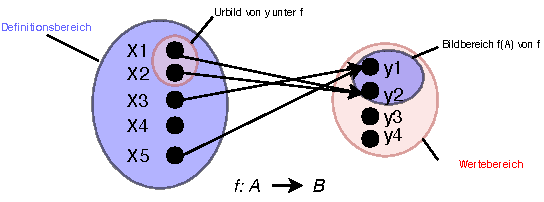
\includegraphics[width=0.95\linewidth]{./begriffe_funktionen.pdf}\\
\textbf{Urbild:} ist Menge\\
$f(x) = x + 1$, testen: $x+1$ auf $\mathbb{R}$ definiert? $\rightarrow$ $x=y-1$: auch auf $\mathbb{R}$?\\
$f(x) = 2x$, $f: \mathbb{N} \rightarrow \mathbb{N}$: Beachten bspw. $y=3$, im Wertebereich aber nicht im Bildbereich.



\subsection{Injektiv, Surjektiv, Bijektiv}
\textbf{surjektiv:} Alle Elemente der Wertemenge $B$ gehören zur Bildmenge $f(A)$:\\
$\forall y \in B \exists x \in A : f(x) = y$, dh. falls $f(A) = B$\\
\textbf{injektiv:} F\"ur zwei verschiedene Argumente $x_1, x_2 \in A$ sind die dazugeh\"origen Funktionswerte $f(x_1)$ und $f(x_2)$ unterschiedlich:\\
$\forall x_1, x_2 \in A : (x_1 \not = x_2 \implies f(x_1) \not = f(x_2))$

Inverse Funktion: $f(x) = 2x$, $(\mathbb{R} \rightarrow \mathbb{R})$, $f^{-1}(x) = 1/2 x$.





\section{Graphen}
\subsection{Begriffe}
\textbf{Kreis:} Wenn $v_{init} = v_{end}$, nicht zwingend jede Kante Teil vom Kreis.

\subsection{Eulergraphen}
Wird in einem Weg jede (!) Kante genau einmal besucht, heisst der Weg Eulerweg.

\textbf{Satz:} In einem Graphen oder Multigraphen kann es nur eine gerade Anzahl von Knoten mit ungeradem Grad haben.

\textbf{Eulerweg I:} F\"ur jeden Eulerweg gilt: jeder Knoten, der nicht End- oder Anfangsknoten, also ``Zwischenknoten'' ist, muss zu einer bisher im Weg unbenutzetn hineinf\"uhrenden Kante eine bisher unbenutze herausf\"uhrende Kante haben.\\
Bei K\"onigsberg: Jeder Knoten hat ungerade Anzahl Kanten, diese k\"onnen alle nicht Zwischenknoten des Weges sein.

\textbf{Notwendige Eulerbedingung f\"ur Eulerwege:} Existiert in einem Graph oder Multigraph ein Eulerweg, dann haben notwendigerweise alle Knoten bis auf zwei einen geraden Grad (also h\"ochstens zwei, bzw. 0 der 2, haben einen ungeraden Grad).\\
$\rightarrow$ \textcolor{red}{Wenn der Graph oder Multigraph zwei Knoten mit ungeradem Grad besitzt, muss der Eulerweg in einem von beiden starten und im anderen enden.}

\textbf{Notwendige und hinreichende Eulerbedingung f\"ur Eulerwege:} Ein Graph oder Multigraph hat genau dann einen Eulerweg, wenn er zusammenh\"angend ist und die notwendige Eulerbedingung erf\"ullt ist, also entweder keinen oder zwei Knoten mit ungeradem Grad hat.

\textbf{Notwendige und hinreichende Bedingung f\"ur Eulerkreis:} Ein Graph hat Eulerkreis, genau wenn er zusammenh\"angend ist und \underline{jeder} Knoten geraden Grad hat.



\subsection{Hierholzer: Berechnung Eulerweg}
\textbf{Input:} Zusammenh\"angender Graph/Multigraph mit maximal zwei Knoten von ungeradem Grad\\
1) W\"ahle beliebigen Startknoten (falls es ungerade Knoten gibt, w\"ahle einen solchen)\\
2) Gehe von diesem Knoten aus \"uber noch nicht besuchte Kanten so lange weiter bis du nicht mehr weiterkommst\\
3) Alle Kanten schon einmal besucht?\\
$\rightarrow$ Ja : Ende\\
$\rightarrow$ Nein: W\"ahle beliebigen Knoten mit noch unbesuchten Kanten auf diesem Weg als neuen Startknoten und gehe zu 2)\\
Wege Zusammengef\"ugt ergeben einen Eulerweg

\subsection{Minimal aufspandender Baum}

``\textit{Greedy}'': In jedem Schritt die beste Wahl treffen, die momentan zur Verf\"ugung steht.\\

\textbf{Von Prim:} ``\textit{In jedem Schritt wird die k\"urzest m\"ogliche Br\"ucke gebaut.}''\\
W\"ahle einen speziellen Ort aus (Festland) und nenne ihn erreichbar.
Alle anderen Orte sind zun\"achst nicht erreichbar.
F\"uhre den folgenden Schritt so oft aus, bis alle Orte erreichbar sind:\\
Baue die k\"urzeste Br\"ucke zwischen zwei Orten, von denen einer erreichbar und der andere nicht erreichbar ist, und nenne den bislang nicht erreichbaren Ort erreichbar.\\

\textbf{Von Kruskal:} ``\textit{Baue in jedem Schritt die k\"urzeste Br\"ucke zwischen zwei beliebige bislang unverbunden Orten.}''\\
F\"uhre den folgenden Schritt so oft aus, bis alle Orte untereinander durch Br\"ucken verbunden sind: Baue die k\"urzeste Br\"ucke, die zwei Orte verbindet, die bisland nicht voneinander aus erreichbar sind.
Beachten: Anfangs sind kann es auch L\"ucken zwischen schon verbundenen Orten geben.

\textbf{Eigenschaften:} Jedes andere Br\"uckensystem wird gesamthaft l\"anger.



\subsection{Matrixdarstellung}
Knoten (Symbole V, v, w) $\rightarrow$ Zeilen\\
\textbf{Adjazenzma., ungerichtet:} $a_{ij}$ = 1, wenn $\{v_i, v_j\} \in E$, 0 sonst\\
\textbf{Adjazenzma., gerichtet:} $a_{ij}$ = 1, wenn $(v_i, v_j) \in E$, 0 sonst\\\\ 
\textbf{Inzidenzma., ungerichtet:} $b_{ij} = 1$ wenn $\exists w \in V: e_j = \{v_i, w \} \in E$, 0 sonst\\
\textbf{Inzidenzma., gerichtet:} $b_{ij} = 1$, wenn $\exists w \in V : e_j = (vi, w) \in E$, $-1$, wenn $\exists w \in V: e_j = (w, v_i) \in E$, 0 sonst

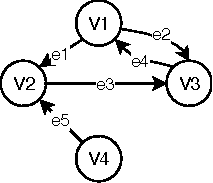
\includegraphics[width=0.5\linewidth]{inzidenz.pdf}

Adjazenzmatrix\\
\begin{tabular}{llll}
0 & 1 & 1 & 0\\
0 & 0 & 1 & 0\\
1 & 0 & 0 & 0\\
0 & 1 & 0 & 0
\end{tabular}


Inzidenzmatrix (Zeilen = Knoten, Spalten = Kanten):\\
\begin{tabular}{lllll}
1 & 1 & 0 & -1 & 0\\
-1 & 0 & 1 & 0 & -1\\
0 & -1 & -1 & 1 & 0\\
0 & 0 & 0 & 0 & 1
\end{tabular}

\subsection{Isomorphismus}
Graphen isomorph unterscheiden sich nur durch Anordnung und Benennung der Knoten.\\
Es existiert eine bijektive Funktion $f: V \rightarrow V'$


\section{\textcolor{red}{Induktion}}

\section{\textcolor{red}{Rekursion}}

Lineare Rekursionsgleichung $k$-ter Ordnung mit St\"orterm:\\
$f(n) = s(n) + \sum_{i=1}^k c_{n-i}(n) \cdot f(n-i)$\\
$s(n)$ St\"orterm, $k$-te Ordnung, $c(n)$ abh\"angige Koeffizientenfunktionen. ``homogen'': St\"orterm $= 0$.\\
$\rightarrow$ Erst durch Angabe von $k$ Anfangsbedingungen $f(1)$, $f(2)$, ..., $f(k)$ eindeutig bestimmt.

\subsection{Rekursionsgraph}
1) Anfangswerte zu Bl\"attern hinzuf\"ugen\\
2) Im Baum aufsteigend f\"ur jeden Vorg\"anger gem. $f$ den Funktionswert ausrechnen und hinschreiben, bis bei Wurzel $f(n)$ angekommen und so den Funktionswert $f(n)$ (die Auswertung) f\"ur das vorgegebene $n$ erhalten



\subsection{Beweis Rekursionsgleichung}

$f(1) = 1$, $f(n) = 1 + 2 \cdot f(n-1)$\\
Nach Tabelle ``\textit{Inhomogene RG 1. Ordg. mit konst. $c$ und konst. $s$''}, somit Ansatz:\\
$\rightarrow f(n) = \underbrace{1}_{a} \cdot {\underbrace{2}_{c}}^{n-1} + \frac{1 - 2^{n-1}}{1-2} \cdot 1$\\

\textbf{Verankerung:}\\
$f(1) = 2^1 - 1 = 2-1 = 1$ gleich Ergebnis Definition Rekursion $f(1)$\\

\textbf{Induktionsschritt:}\\
$A(n-1) \implies A(n)$\\

\textbf{Annahme:}\\
$f(n-1) = 2^{n-1} - 1$ (besser, weil in RG auch $f(n-1)$ steht)\\

\textbf{Behauptung:}\\
$f(n) = 2^n - 1$\\

\textbf{Beweis:}\\
$f(n) = 1 + 2 \cdot f(n-1) \stackrel{\mbox{Ann.}}{=} 1 + 2(2^{n-1} - 1) = 1 + 2^n - 2 = 2^n -1$\\


% $f(1) = 1$\\
% $f(n) = 4 \cdot f(n-1) + 4^{n-1}$, f\"ur $n \in \mathbb{N}$ mit $n \geq 2$.\\
% $\rightarrow$ $f(n) = 4^{n-1} \cdot n$.\\
% \textbf{Annahme:} $f(n-1) = (n-1) \cdot 4^{n-2}$\\
% \textbf{Behauptung:} $f(n) = n \cdot 4^{n-1}$ f\"ur rekursive Formel\\
% \textbf{Beweis:}\\
% $f(n) = 4 \cdot f(n-1) + 4^{n-1} = 4 \cdot (n-1)\cdot 4^{n-2} + 4^{n-1} = \dots = 4^{n-1} \cdot n$\\

\textbf{Beweis durch Einsetzen:}\\
1) Gilt die explizite Darstellung der Zahlenfolge f\"ur $n=1$\\
2) Ist die Gleichung korrekt, wenn die explizite Darstellung in die rekursive Definition eingesetzt wird?\\
$\rightarrow$ Explizite L\"osung $f(n) \stackrel{?}{=}$ Gleichung gem. Rekursionsdef. $f(n) = s + c f(n-1)$






\end{multicols}
\subsection{Rekursionsgleichungen}
\begin{tabular}{lll}
\hline
Homogene RG 1. Ord.                                            & $f(n) = c(n) \cdot f(n-1)$ mit $f(1) = a$, $a \in \mathbb{R}$ & Iteration: $f(n-1)$, $f(n-2)$, ... einsetzen \\
Homogene RG 1. Ord. mit $c=c(n)$ konst.                        & $f(n) = c \cdot f(n-1)$ & $f(n) = a \cdot c^{n-1}$ \\
Inhomog. RG 1. Ord.                                            & $f(n) = s(n) + c(n) \cdot f(n-1)$, $f(1) = a$ & $f(n-1)$, $f(n-2)$, ... einsetzen \\
Inhomog. RG 1. Ord. mit konst. $c=c(n)$ und $s=s(n)$           & $f(n) = c \cdot f(n-1) + s$, $f(1) = a$, $a \in \mathbb{R}$ & $c \neq 1$: $f(n) = a \cdot c^{n-1} + \frac{1 - c^{n-1}}{1-c} \cdot s$ (\textbf{Achtung:} St\"orterm!)\\
& & $c = 1$: $a + (n-1) \cdot s$ \\
Inhomog. RG 1. Ord. mit konst. $c=c(n)$ und allgm. $s(n)$      & $f(n) = s(n) + c\cdot f(n-1)$, mit $c \in \mathbb{R}$ und $f(1) = a \in \mathbb{R}$ & $f(n) =$ ``\textit{allg. L\"osung der dazugeh. homog. Gleichung}'' $+ p(n) = d\cdot c^{n-1} + p(n)$\\
             & & $d \in \mathbb{R}$, $p(n)$ spezielle (partikul\"are) L\"osg. der inhomog. Rekursion, und\\
             & & \textcolor{red}{nicht} L\"osung der zugeh\"origen homogenen Gleichung \\
Homog. RG 2. Ord. mit konst. $c_1 = c_1(n)$ und $c_2 = c_2(n)$ & & \\
Inhomog. RG 2. Ord. konst. $c_1 = c_1(n)$ und $c_2 = c_2(n)$ und allgem. $s(n)$ & & \\
Nicht linear, 1. Ord. & $f(n) = 2 \cos (f(n-1))$, $f(n) = f(n-1)^2$ & \\\hline
&&\\\\
\end{tabular}




\setlength{\columnsep}{1cm}
\begin{multicols}{3}


\subsection{Vorgehen Bestimmung Explizite Darstellung}
1) Zahlenbeispiele mithilfe rekursiver Darstellung\\
2) Induktives Schliessen\\
3) Vermutung f\"ur explizite Darstellung\\
4) Vollst\"andige Induktion oder Einsetzen\\
5) Explizite Darstellung

\subsection{Ans\"atze für $s(n)$:}
\begin{tabular}{ll}
$s(n)$ & Ansatz f\"ur $p(n)$ \\\hline
6      & $x$ \\
$n$      & $xn + y$ \\
$n^2$    & $xn^2 + yn + z$\\
5$^n$    & $t \cdot 5^n$ \\
$n \cdot 7^n$ & $(xn + y) \cdot 7^n$ \\
$n^2 \cdot 7^n$ & $(xn^2 + yn + z) \cdot 7^n$ \\\hline
\\
\end{tabular}

\textbf{Zugeh\"orige homogene Rekursionsgleichung:}\\
$f(n) = s(n) + \underbrace{\sum_{i=1}^k c_{n-1}(i) \cdot f(n-i)}_{= h(n)}$\\
$h(n)$: ``\textit{zugeh\"orige homogene Rekursionsgleichung}''.\\
\textbf{\textcolor{red}{Achtung:}} $h(n) = \sum_{i=1}^k c_{n-i}(n) \cdot \textcolor{red}{h}(n-i)$

\end{multicols}



\end{document}
